
With simplified IR groups through BSF simplification, \phoenix\ further performs a \emph{Tetris-like IR group ordering} procedure targeting a global circuit-depth optimal arrangements of IR groups. We abstract the circuit structure exhibited by each simplified IR group, excluding all 1Q operations (e.g., local Pauli rotations), such that assembling two subcircuits is like assembling two Tetris. Therefore, we quantitatively characterize the assembling procedure by defining uniform Tetris-regarding data structures of subcircuits and a uniform cost function, with gate cancellation opportunities and qubit routing overhead further taken into account:
\begin{enumerate}
    \item \textit{Uniform empty endian vectors of circuits and the depth overhead metric.} As shown in \Cref{fig:empty-end} (a), we define a pair of vectors $e_l$ and $e_r$ for each circuit, named \dquote{left-empty-end} and \dquote{right-empty-end} vectors, respectively. The $i$-th entry of $e_l$ ($e_r$) refers to the wire depth where the first 2Q gate acting qubit $i$, looking from the left (right) side. % It is calculated by layering the circuit in its directed acyclic graph (DAG) according to the nodes' topological orders.
    By means of this definition, the depth overhead for assembling two subcircuits can be rigorously quantified as
    \begin{align*}
        \mathrm{cost}_\mathrm{depth} :=  
                \left\{
                \begin{array}{ll}
                \textsc{sum}(\eRrightPre + \eLeftPost),  \text{ if } \textsc{all}(\eRrightPre[\eLeftPost == 0] > 0) \\\qquad \text{    }\qquad\text{    }\qquad\text{   }\text{and }\textsc{all}(\eLeftPost[\eRrightPre == 0] > 0) \\
                \textsc{sum}(\eRrightPre + \eLeftPost - 1), \text{ otherwise    }
                \end{array}
                \right.
    \end{align*}
    corresponding to two Tetris assembling scenarios in \Cref{fig:empty-end} (b).
    \item \emph{Consideration of Clifford2Q cancellation.} The simplified IR group usually exposes Hermitian Clifford2Q operators at the two ends of the subcircuit. Therefore some Clifford2Q gate cancellation opportunities could be exploited, which does or does not further induce circuit depth decrease of the preceding and the succeeding subcircuits, as depicted in \Cref{fig:gate-cancel} (a). We integrate their impact into $\mathrm{cost}_\mathrm{depth}$: (a) if $m$-pair Clifford2Q cancelled without depth decrease, $\mathrm{cost}_\mathrm{depth} \gets \mathrm{cost}_\mathrm{depth} - 2m$; (b) if with one-side circuit depth decrease, $\mathrm{cost}_\mathrm{depth} \gets \mathrm{cost}_\mathrm{depth} -2m -n$; (c) if with two-side circuit depth decrease, $\mathrm{cost}_\mathrm{depth} \gets \mathrm{cost}_\mathrm{depth} - 2m -2n$.
    \item \emph{Consideration of qubit routing overhead.} The hardware-aware compilation usually results in considerable 2Q gate count overhead during the qubit mapping stage which inserts necessary $\SWAP$ gates to rout qubits within the connectivity-constrained topologies. The key idea of co-optimization for qubit routing is to minimize the mapping transition overhead between assembled subcircuits. \phoenix\ aims to tackle it in a high-level heuristic approach, not limited to specific routing schemes (e.g. three-$\CNOT$ unrolling of $\SWAP$, bridging gate) and hardware topologies. Intuitively, two subcircuits with more \dquote{similar} qubit interaction behaviors require less mapping transition overhead between them, as demonstrated by \Cref{fig:gate-cancel}. Therefore, we introduce a factor characterized by the similarity between the qubit interaction graphs of two circuits to scale the uniform depth overhead function,
    \begin{align}
        \mathrm{cost}_\mathrm{depth} \rightarrow s \cdot \mathrm{cost}_\mathrm{depth},\quad s = \sum_i \frac{D_i\cdot D_i'}{\lVert D_i \rVert_2 \lVert D_i' \rVert_2},
    \end{align}
    where $D$ ($D'$) is the distance matrix of the preceding (succeeding) subcircuit's qubit interaction graph in which $D[i,j]$ represents the shortest path length between qubit $i$ and qubit $j$. The similarity calculation is like the cosine-sine similarity metric, reflecting the similarity of both global topological structures and qubit-wise local topologies.
\end{enumerate}


\begin{figure}[tbp]
    \centering
    % \subfigure[Clifford2Q cancellation.]{
    %     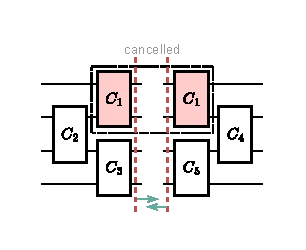
\includegraphics[width=0.46\columnwidth]{figures/gate_cancel_1.pdf}
    % }
    % \subfigure[Clifford2Q cancellation with reduced depth.]{
    %     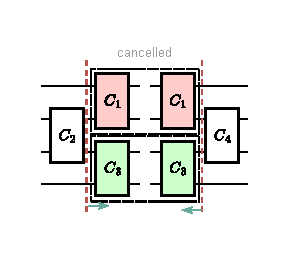
\includegraphics[width=0.46\columnwidth]{figures/gate_cancel_2.pdf}
    % }
    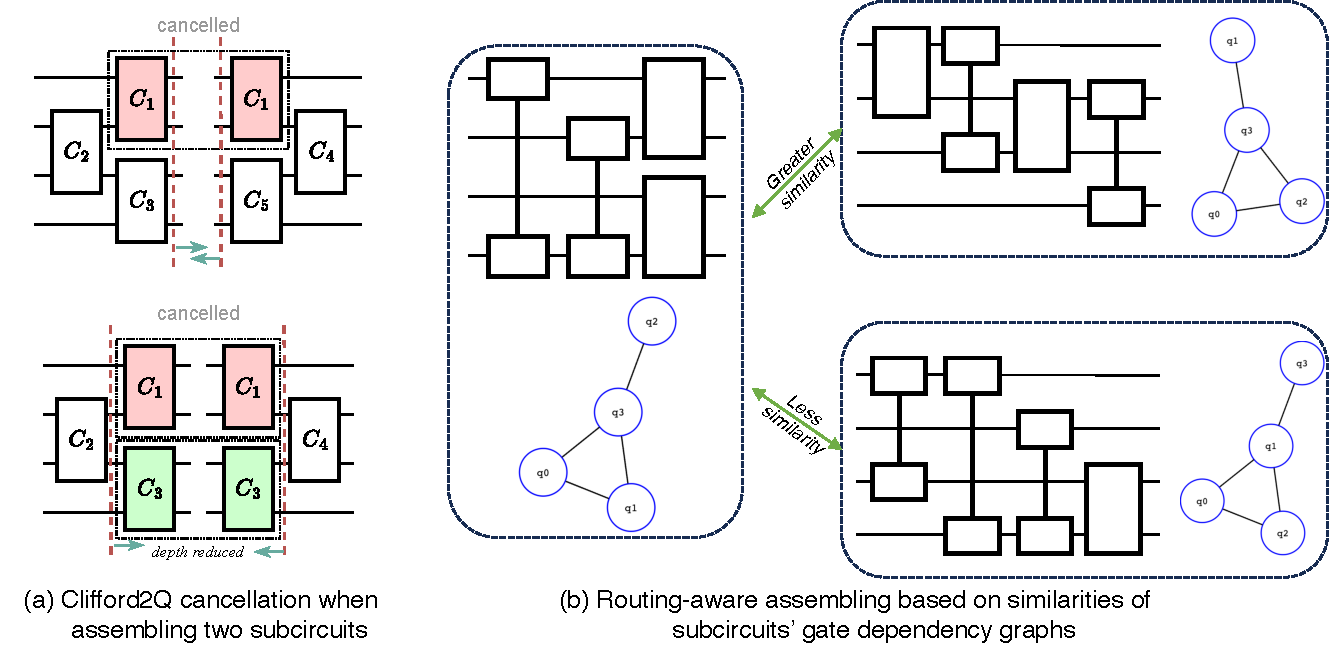
\includegraphics[width=\columnwidth]{figures/gate_cancel.pdf}
    \caption{Clifford2Q gate cancellation opportunities. Routing-aware assembling.}
    \label{fig:gate-cancel}
\end{figure}

In practice, these IR groups are first pre-arranged in descending order of their weight (subcircuit width). \phoenix\ lookahead for a certain number of subcircuits, to determine which one is to be appended by the current tail subcircuit by comparing their respect $\mathrm{cost}_\mathrm{depth}$ with the tail subcircuit. This process iterates until all subcircuits are assembled. Overall, the Tetris-like IR group ordering strategy exhibits a globally depth-optimal ordering scheme under the guidance of uniform cost metrics, aware of both gate cancellation benefits and qubit routing overhead.







\caption{Gate cancellation opportunities and routing-aware assembling.  (a) Clifford2Q cancellation between the preceding and succeeding subcircuits may or may not induce circuit depth decrease.  (b) The subcircuit (upper right) whose qubit interaction graph is more similar to that of the already assembled subcircuit (left) is preferred than the other (lower right).



        
when choosing whether assmbling subcircuit 1 or subcircuit 2 to .......,  opportunities when assembling two simplified IR groups. Routing-aware assembling. \ZY{Make this figure caption more detailed}}